\documentclass[11pt]{article}

\usepackage[utf8]{inputenc}
\usepackage{graphicx}
\usepackage{amsmath}
\usepackage{hyperref}
\usepackage{listings}
\usepackage{geometry}
\usepackage{xcolor}
\usepackage{enumitem}
\usepackage{amsfonts}
\usepackage{tikz}
\usetikzlibrary{calc}

\geometry{
    letterpaper,
    margin=1in
}


\title{The Federated Open Key Service (FOKS)}
\author{Maxwell Krohn (max@ne43.com)}
\date{\today\\Version 1.4}


\begin{document}

\newcommand{\yubi}{Yubikey}
\newcommand{\Yubi}{Yubikey}
\newcommand{\yubis}{Yubikeys}
\newcommand{\Yubis}{Yubikeys}

\maketitle

\begin{abstract}

This paper presents FOKS (Federated Open Key System), a
decentralized key management system designed to provide secure and flexible key
distribution across federated networks. The basic problem addressed is that 
of two parties sharing end-to-end encrypted data across the internet, where both
parties have several devices. They might rotate devices, form mutable teams with
other users, or even teams of teams in an arbitrary graph. They need to share
secret key material to facilitate symmetric encryption, and this material must
rotate whenever devices are replaced, or team membership changes.  This is a
very natural problem but one that still lacks an adequate solution.  Moreover, we
believe key management should not lock users into a particular, walled provider,
but instead, should allow for federation and independent management of server
resources, as we see in HTTP and SMTP.  We describe the system architecture,
security model, and implementation details of a system that achieves secure,
federated key exchange, and enables useful applications like end-to-end
encrypted data sharing and git hosting.

\end{abstract}


\section{Introduction}

In recent years, Signal, iMessage and WhatsApp have proven out the customer
demand for end-to-end encryptied communication. But despite the success of these
systems, and their vast improvements over previous, less-secure systems,
important problems remain unresolved.  Most obviously, questions remain around
identity. In a recent, high-profile incident, United States government officials
misused Signal to mistakenly leak matters of national security to the
press~\cite{signal-hesgeth-leak}. Relying on phone numbers as identifiers is
only part of the problem; the larger issue, arguably, is that public identities
are hard to audit and map to public keys, and that large groups are even harder
to manage.

We see other issues: all the systems mentioned above and many others lock users
into a walled-garden with a centralized single provider. Outside observers lack
the ability to experiment with their own servers as part of a security audit.
Many of these systems lack an unconditional commitment to open-source
everywhere, closing off parts or all of their systems to third party scrutiny. 
Single-provider systems further suffer from vendor lock-in. As data is not
portable, and switching to a competing platform is not supported, the service
providers have the leverage to ``monetize'' their users as they see fit.

The authors have deep experience with the Keybase system~\cite{keybase}, which
came at these problems from a different angle. In Keybase, the initial focus was
on identity, multi-device support, and formation of auditable groups that could
evolve over time. But Keybase shows the same limitations as Signal, WhatsApp and
iMessage: it is stuck on a single-provider model.

This paper introduces a new system: the Federated Open Key Service (FOKS).  It
inherets much from these prior system but inhabits a different point in the
design space. FOKS provides secure key distribution for users who have multiple
devices. It allows those users to form groups, and unlike previous systems, for
those groups to join other groups. Whether managing a user's device cloud, or
managing the membership of a team, FOKS ensures that a malicious server cannot
inject invalid members, and that it cannot withhold important revocations and
deletions.  Many of these features are possible with previous systems, but
FOKS's major architectural advance is the support of federation. Anyone
can run a server in the FOKS network. Users can stay siloed on different
servers, or can form teams that span multiple servers. Federation gives users
more choice, control and better guarantees. Though servers cannot decrypt or
sign on behalf of users, they still can see metadata, and often are called upon
to protect user privacy. Therefore, companies or tight-knit groups have
good reason to run their own servers, and can do so in the system.

The aim here is to build a general protocol that can scale to the internet, 
owned by no single party. FOKS aims to be agnostic to hosting provider, much
like SMTP or HTTP. What those protocols have done for email and the web, FOKS
aims to do for cryptopgrahic key management and distribution.

This paper introduces and describes the FOKS system. We cover a threat model
in Section~\ref{sec:threatmodel}, a system design in Section~\ref{sec:design}, 
the use of cryptography in Section~\ref{sec:crypto}, and some important applications
in Section~\ref{sec:apps}. The primary goal here is not academic novelty, but
rather to describe a system that embodies a unique
and quite useful set of trade-offs for end-to-end encrypted systems.
However, there are some, to our knowledge, new contributions:
%
(1) An exploration of key-rotation for teams that can form
      nearly arbitrary graphs across federated servers;
%
(2) a system for hiding identity and team updates in a larger
      transparency tree without the need
      for pseudo-random functions; and
%
(3) a new protocol specification language (called Snowpack) that enforces
  domain separation for cryptographic operations.



\section{Threat Model}
\label{sec:threatmodel}

In FOKS, we consider a threat model similar to that of the Keybase~\cite{keybase},
SEAMLess~\cite{chase2019seemless} or CONIKs~\cite{melara2015coniks} systems.
The high level north star is end-to-end secrecy and integrity. Only the clients
at the edges of the system should be able to decrypt important data, and only
those clients can make authorized changes to the data. Of course, multiple
devices per user and mutable groups complicate the picture.

We assume that clients are trustworthy, and behave properly. If this assumption
is violated, say, if a client is compromised by a rootkit, then we cannot
offer any guarantees. 

Users might sometimes lose their devices. In an ideal world, hardware protections
would prevent whoever recovered the device from accessing the device's private
key material. In the case of hardware keys (like YubiKeys), or backup-keys
written on paper, the user has less protection during comrpomise. Regardless,
once the user revokes the lost device, keys should rotate so that data is secure
going forward (this property is known post-compromise security). In some cases,
past data might be safe from the attacker (this property is known as forward-secrecy).
but the specifics depend on the trustworthiness of the server (see below). Similarly, revoked
keys on lost devices lose their signing power, and other devices will not accept
their signatures going forward.

The threat model is here is similar but not exactly the same as Signal's and
WhatsApp's, because our applications feature persistent (rather than ephemeral)
data. If a new user joins an existing group, or if a user adds a new device,
they should be able to access old data, which might be required to reassemble the
shared resource. For instance, when Alice adds Bob to a git project, Bob
should see all past commits in the commit history, otherwise the
application will break. Thus, we can't guarantee foward-secrecy, since
lack of forward secrecy is needed for the application to function properly.

In FOKS, clients pick their servers. They might select for servers
that are generally aligned with. They can run their own servers, or pick 
from third party hosting providers. Users should assume that servers
are generally trustworthy, but might suffer comrpomises from time to time.
For instance, servers might be running on cloud infrastructure, and the underlying
storage, network, or computation might be compromised. Insiders or state actors
might have privileged access to the underlying infrascture. 

If servers behave honestly, the FOKS system works securely as expected.  If
servers behave maliciously, they can deny access to data through a variety of
mechanisms: they can go offline, they can withoold data, or they can subtly
current server-resident data to confuse clients. In this last case, the system's
security design should prevent the clients from leaking secrets or accepting
unauthorized changes to data. But as in the other more obvious cases, the
clients will lose access to their data.

When servers are behaving honestly, they can provide clients with
forward-secrecy. That is, if honest servers throw away data encrypted with old
keys, an attackets with access to private keys cannot rcannot ecover past data.
This property is an improvement over that offered by the Keybase system, which
assumed the worst in the case of a comrpomise. If we assume on the other hand
that an attacker who steals a private key operates in cohoots with the server,
then we cannot offer any guarantees about forward secrecy.

Servers do not trust each other. If one server becomes corrupted, it has no
bearing on the other servers in the system. In other words, we assume attackers
can stand up their own servers, since anyone in the system can do so.


% Introduction content goes here


\section{Design}

FOKS is a classic client-server system. At a hight level, the clients
manage private keys, and the server manages public keys, encryptions of, 
shared secret keys, and encrypted data. Users generally trust their
servers to be online, available and not to intentionally sabotage
agreed-upon protocols. 

\subsection{System Architecture}

Much like HTTP or STMP, FOKS clients communicate with one or more servers,
depending on where users have accounts. They can safely ignore the other servers
in the system. Most communication is between client and server, and there is
little if any server-to-server or client-to-client communication.  This
property simplifies protocol upgrades and network configuration.

Each client can speak for many users, as users can have accounts on different
servers, or several accounts on the same server. By analogy, an email client can
server multiple emails accounts for the same user concurrently, say one for work
and one for personal use. Or a web browser might have different personae (with
different cookies, preeferences, passwords and history) for the same user.

Each of the users can of course have multiple devices, like a desktop, a laptop,
a phone, and a \yubi . Additionally, users can have "backup devices", which can
be writted down on paper and stored in a safe place. The system recommends at
least two devices to prevent data loss. That is, these devices have private keys
that decrypt data, and the loss of the last key prevents decryption of the data.
Obviously there is a trade-off here: the more devices, the more likely the user
will lose one, or have one stolen; the fewer devices, the more likely the user
will lose all devices and therefore access to data. Some optimal middle ground
exists, but varies with the users and their behaviors. 

\subsection{Key Hierarchy}

The FOKS key hierarchy sits at the core of the system. It aims to provide users
with a sequence of symmetric keys shared across all of their devices, so that
they can store data encrypted with the latest key, and can decrypt (and
authenticate) data encrypted with older keys when necessary. Similarly, users in
a team should share secret keys that users outside their teams cannot see, allowing
them to share encrypted data via untrusted FOKS servers.

\subsubsection{Device Keys}

When a user sits down at a FOKS client to signup or provision a new device
for an existing account, she first creates a new key-pair specifically
for that device. The private key never leaves the device. She shares the public key
with the FOKS server, who eventually selectively shares it with user users.
We detail the exact cryptography in Section~\ref{sec:cryptography}.

Hardware keys that support the PIV protocol (like \yubi{} version 5 and later)
can also be used as device keys. These devices get randomly-generated private
keys in the factory, written to one of 20 possible "slots." FOKS users select
a slot to use, and the client sends the corresponding public key to the FOKS 
server. Signing and decryption operations happen on the device against the chose
slot. 

\subsubsection{Per-User Keys (PUKS)}

Every user on the FOKS system has one of more per-user keys, or PUKS. A PUKS
is a randomly-generated key-pair whose private key is encrypted for each of
the device public keys. This way, all current devices can access the current
PUK secret key, and perform decryptions or signatures for the current PUK public
key. The client makes a new PUK every time the user revokes a device. The system
encrypts the old PUK secret keys for the new PUK secret key. This way,
a device that has access to the latest PUK can get access easily to all prior
PUKs.

Once the PUK sequence is estblished, the system has a convenient way to encrypt
a data for all of the user's device --- it simply encrypts the data for the 
user's latest PUK.

\subsubsection{Per-Team Keys (PTKs)}

Each team has a sequence of per-team-keys, or PTKs, which are analogous
to PUKs for users. Upon creation, a team gets a new random PTK. The 
client performing the creation sends the public part of the PTK to the server.
The private part of the PTK is encrypted for each member's latest PUK,
and therefore is available on each of the user's devices.

As with PUKs, data that the team shares is encrypted for the team's latest PTK,
and all members can decrypt it. As we will see in Section~\ref{sec:teams}, teams can
join other teams, but the key hierarchy works just the same. When team $A$ joins
team $B$, the secret part of team $B$'s PTK is encrypted for team $A$'s latest PTK,
so that all members of team $A$ can decrypt $B$'s PTK, and therefore, all of
$B$'s encrypted data.

\subsection{Key Roles}

\newcommand{\owner}{\textsf{owner}}
\newcommand{\admin}{\textsf{admin}}
\newcommand{\reader}{\textsf{reader}}
\newcommand{\none}{\textsf{none}}
\newcommand{\role}[1]{\textsf{role}(#1)}


FOKS has a notion of a ``role'' for device keys, PUKs and PTKs. The roles
are: \owner, \admin, and \reader, but \reader{} keys have a "visibility level"
that varies between -32768 and 32767. There is a total ordering among key roles,
so that $\owner > \admin > \reader$, and between reader keys, $k_1 > k_2$ iff
$k_1$ has a higher visibility level than $k_2$.

The important property enforced is that we only encrypt PUK $k$ for device key
$j$ if $\role{k} \le \role{j}$, and similarly, we only encrypt PTK $k$ for PUK
$j$ if $\role{k} \le \role{j}$.

The idea here is that the owners of a group get to see all the keys; the admins
can see the admin and reader keys; and the readers can see keys at or below
their visiblility level. This configuration allows groups to have
lower-privileged members, and for users to have lower-privileged devices. At
Keybase, a similar but less-flexible property allows ``bots'' into teams, so that
all the members of the teams can interact with the bots, but the members had
channels to communicate that the bots aren't privvy to.  For now, all user
devices are at the \owner{} role, but we plan to relax this requirement in the
future.

\subsection{Data Structures}

We now have some basic motivation as to what the key system ought to achieve.
It ought to allow groups of devices, groups of users, or groups of users
and teams to share a secret encryption key. From there, they can share data
encrypted (and authenticated) with that key. But the question becomes,
how are users formulated from devices, and how are teams formulated from users
so that only desired members are in the group, especially if the server
behave maliciously?

For instance, a malicious server might fool a user into encrypting secret data
for an invalid device, or team administrator into encrypted data for an invalid
user.

\subsubsection{Signature Chains}
\label{sec:sigchains}

FOKS uses the same mechanism as Keybase here --- the signature chain (or
``sigchain'' for short).  The sigchain is a series of signed statements that
form a cryptographic chain, meaning they can only be replayed in the intended
order. Replaying the chain allows a viewer to confirm the chain appears how the
author intended and wasn't tampered with, even if the set of signers varies over
time. Of course, signers do vary over time as users add and remove devices, or
as they add and remove members from teams.

Each user (and team) gets its own sigchain. The sigchain keeps an indellable record
of which keys can update the chain, and which PUKs or PTKs are currently
active for the user (or team).

\paragraph{Users} The first link in a sigchain is called the ``eldest'' link. For user sigchains,
the first device generates this link, generates the first PUK, and then computes
a signature over the following data:

\begin{enumerate}[label=U.\arabic*]\itemsep0em
    \item \label{item:prev} The hash of the previous link in the chain (nil for the eldest)
    \item The current sequence number of the sigchain (which is 1 for the eldest link)
    \item A commitment to the next random tree location (see Section~\ref{sec:location-hiding})
    \item The current Merkle root hash (see Section~\ref{sec:merkle})
    \item The user's ID and the server's host ID (see Section~\ref{sec:hostchains})
    \item \label{item:puk} The user's new PUK public keys
    \item The user's new device key
    \item A ``subchain tree location seed commitment`` (see Section~\ref{sec:subchains})
      \label{item:stlsc}
    \item A cryptographic commitment to the user's username (see Section~\ref{sec:naming})
       \label{item:name}
    \item A cryptographic commitment to the user's device name (picked by the user)
    \item The role of the new device (currently always \owner ).
    \item For \yubis , a public ``subkey' used to authenticate the client
      to the server.
\end{enumerate}

The client computes nested signatures first by the new PUKs introduced in
Step~\ref{item:puk}, and lastly by the user's device key. (Recall that sometimes
several PUKs can be introduced at once due to the different possible device
roles). The client uploads the whole package as the user's eldest link.

Subsequent links proceed in largely the same way, with a few minor differences.
The previous hash (\ref{item:prev}) is the collision-resistent hash of the 
package uploaded in the previous step. In some cases, like device addition,
new PUK public keys (\ref{item:puk}) do not appear. In these cases,
no signatures with PUKs are required.

For any link in the chain, a set of devices is authorized to make further
updates to the chain. After the first link, the set contains only the first
device (sometimes called the ``eldest`` device). A link can either add a new
device, or revoke an existing device, updating the set of authorized devices
accordingly. When clients upload new chainlinks, the server enforces valid
signatures by authorized devices. When users replay this chain, they perform the
same check. This simple mechanism ensures the server can't introduce a bogus
device.

\paragraph{Teams} A team chain link contains the following fields, many of which
are analagous to user chains:

\begin{enumerate}[label=T.\arabic*]\itemsep0em
    \item The hash of the previous link in the chain (nil for the eldest)
    \item The current sequence number of the sigchain (starting at 1)
    \item A commitment to the next random tree location
      \label{item:next-tree-location}
    \item The current Merkle root hash 
    \item The team's ID and the server's host ID
    \item The user (or team) ID, host ID, and PUK (or PTK) of the actor making the change
       \label{item:team-actor}
    \item New PTK public keys
    \item \label{item:membership} A set of membership changes
    \item A ``subchain tree location seed commitment``
    \item A cryptographic commitment to the team's name (optional if not changing)
    \item The team's ``index range'' (see~\ref{sec:team-index-range})
\end{enumerate}

Since teams can contain both users and other teams, the actor creating or
modifying the team can be either a user or a team. In FOKS, a \textit{party}
refefes to someone or something that can be in a team, so either a user or a
team. In field~\ref{item:team-actor}, the link contains the unique identifier of
the party (which is the user or team ID plus the host ID), and also the key
making the change. For users, this key is the user's latest PUK at the \owner{}
role.  For teams, it's the team's latest PTK at the desired source role. That
is, consider a teams $T$  where users $a$ and $b$ are owners of $T$, $c$ is an
admin and $d$ is a reader (at visibility level 0). If $T$ creates a new team $U$
with source role of \owner, then only users $a$ and $b$ will have access. If
$T$ creates the new team with source role of \reader, then all users will have
access. 

FOKS clients and servers enforce these access controls with the key hierachy.
In the case of the owners of $T$ creating $U$, $T$'s \owner{} PTK appears in
field~\ref{item:team-actor} and performs the signature over the chainlink. 
As $T$ creates $U$, it makes new PTKs for $U$. It encrypts the secret keys
of these new PTKs for the \owner{} PTK of $T$. This way, everyone in the owner
group of $T$ can now access $U$'s PTKs. The second example follows similarly,
with the readers of $T$ getting access to $U$'s secret PTKs after team creation.

The membership changes field (\ref{item:membership}) contains the following
fields for each member being modified:

\begin{enumerate}[label=M.\arabic*]\itemsep0em
    \item The ``destination role'': the role the member is to have in the team; for removals,
      this is the role \none .
      \label{item:dst-role}
    \item The member's party and host IDs (a party ID is a user ID or a team ID).
      \label{item:party-id}
    \item The source role: the role the member has in its current party.
    \item The member's public PTK or PUK from its current party.
      \label{item:team-member-ppk}
    \item The generation number of that PTK or PUK.
    \item A commitment to a ``team removal key'' (see Section~\ref{sec:removal-keys})
\end{enumerate}

In the case of team creation, member addition, member role upgrade or downgrade, the
role in field~\ref{item:dst-role} is the new role in the target team that the member
has after the change is applied.  In the case of removal, the role is \none. 

Note that in field~\ref{item:team-member-ppk}, the public PUK (or PTK) appears directly
in the chain, in addition to the ID of that party. Admins and owners are later allowed to
make team modifications, and these are the public keys that will sign these modifications.
Team readers in particular might lack the permission to load the chains of these users
and teams directly, so it's crucial the keys appear directly in the team chain. 
See Section~\ref{sec:sigchain-viz} for further details about sigchain visibility.

As alluded to above, owners have ultimate control over the team. They can add and remove
members, add other owners, downgrade owners to admins, etc. Admins have more limited 
control; the have similar control over admins and readers, but cannot: upgrade admins
to owners, introduce new members as owners, remove existing owners; or downgrade 
existing owners. Readers cannot make any team modifications but can of course read
team chains, and can access data protected by the reader's PTKs at their level
and below.

Teams, unlike users, can include members located on different servers. Above, in 
item~\ref{item:party-id}, we include the host ID of the party in the membership change.
Remote members cannot be admins or owners, but can be readers. This configuration allows
for convenient data sharing across federation boundaries, but simplifies team management
relative to an alternative system where remote members can be owners or admins.

Parties making changes to team sign new team chain links much the same way as user devices
sign user chain links. First, all new PTKs sign the chain link, and then the acting
party's latest PUK or PTK signs the chain link. This PUK or PTK must be the exact key
advertised earlier in the chain in the case of link 2 and above. The eldest link
is essentially self-signed.

\subsubsection{Sigchain Playback}

Whenever a client on the time interacts with another party, or even itself, it
begins by playing back that party's sigchain. The client connects to the party's home
server, downloads any new links it hasn't seen, and ensures the new links play back
cleanly on top of links it previously cached. The rules for playback are largely
implied by the discussion above, such as:

\begin{itemize}\itemsep0em
    \item All chains start at 1, and have ascending sequence numbers.
    \item All links should contain the hash of the previous link.
    \item All links should have valid signatures by devices, PUKs or PTKs that the chain 
      itself authorized. Eldest links are essentially self-signed.
    \item The role restrictions described in Section~\ref{sec:sigchains} are obeyed in team chains.
\end{itemize}

Once playback succeeds, the client has a set of devices keys, PUKs and PTKs that can
speak on behalf of the party. It also has rosters of devices of members who share that
key. From here, useful application work can take over. For instance, in the case
of file sharing (whether via Git or via a KV-store interface), a key derived from the
most recent PUK or PTK serves as the symmetric key for authenticated encryption. 
Whenever the PUK or PTK rotates to a new generation, future encryption should use the
new key.

\subsubsection{Merkle Tree}
\label{sec:merkle}

Section~\ref{sec:threatmodel} describes the FOKS threat model, and we assume the
server can behave maliciously.  Sigchains prevent a server from creating new
chainlinks out of whole cloth and interleaving those with legitimate links. The
protection simply is that the server does not have the private keys the parties
use for signing. We assume those never leave the devices they are made on. By these 
mechanisms, the server cannot extend a chain or replace an inner link. The server can
of course create a brand new chain, and might attempt clients into using this chain
rather than the one the users intended. This case of "mistaken identity" is one
of \textit{naming}, which we cover in Section~\ref{sec:naming}.

The server can nonetheless \textit{withhold} links at the end of a chain, 
or show some clients the full chains, and other various subchains, with the
hope of forcing them to ``fork'' the sigchain into 2 incompatible directions.
We need a mechanism to force the server's hand into showing a consistent 
chain tail to all users who request it. This is where the Merkle tree
comes in. FOKS servers expose a Merkle Tree that forces the server to commit
to a coherent state of the system, across all parties, preventing selective
rollback of sigchains. 

FOKS uses a Merkle Tree strategy that is a hybrid of Keybase's~\cite{keybase},
CONIK's~\cite{melara2015coniks} and SEEMLess's~\cite{chase2019seemless}, but
with a simple novel mechanism introduced to obviate the need for pseudo-random
functions. The Merkle tree stores each party's sigchain tail at a leaf 
in the Merkle tree. The server computes hashes all the way up to the root node.
The \textit{root block} contains this tree root hash, a pointer to the previous version of
the tree (called the previous ``epoch''), a logarithmicly-sized set of pointers
to previous roots further back in history, and also the tail of the 
server's hostchain (see Section~\ref{sec:hostchains}). The hash of this
root block is now a summary of the entire system. The server attempts to publish
root blocks immediately after every sigchain update, but sometimes batches 
them for efficiency. In general, roots should be produced no more than
15 seconds after a sigchain update to keep clients responsive (since sometimes
they need to wait for updates).

\subsubsection{Root Chaining}

Since many users and teams might be active on a signle FOKS server, 
the user has no reason to download every root Merkle epoch. Rather,
the user will experience long gaps between epochs, especially if going
periodically offline. Whenenever a client downloads a root block,
say at epoch $i$, it writes it to local storage. When the client later
downloads another root block, call it $k$, the client enforces
that $i < k$. It also sends up the paremeter $i$, and the server
replies with intermediate blocks $j_1, j_2 \dots j_n$, such that
$i < j_1 < \cdots j_n < k$,  where block $j_{a}$ contains
a pointer to $j_{a-1}$, block $j_1$ contains a pointer to $i$
and block $k$ contains a pointer to $j_n$. The spacing of the
previous pointers in the root block ensures than $n$ is appromixately
$\log (k-i)$. Chaining root blocks in this way 
encourages the server to maintain a consistent, coherent append-only
tree. Clients should perform periodic audits of all root blocks
to ensure previous-pointer consistency across all epochs.

\subsubsection{Location Hiding}
\label{sec:location-hiding}

For the party $p$, at sequence number $i$, the leaf node is a key-value pair,
where the key is $H(p,i,t,r_i)$, and the value is the hash of the signature of
the last link in the sigchain (the $i$th). $t$ is an enumerated value that
specifies which type of chain for $p$ this is. As we will see in 
Section~\ref{sec:subchains}, each party has multiple chains.  $r_i$ is a random
value that was generated when the $(i-1)$ link was published. The $(i-1)$ link
contains the value $H(r_i)$ in the field~\ref{item:next-tree-location} from
Section~\ref{sec:sigchains}. This simple mechanism achieves the same end as the
PRF in CONIKs and SEEMLess, in that it's unpredictable in the tree where a
team's sighcains is stored. This unpredictability prevents data leaks that would
otherwise allow the owners of neighboring nodes in the tree to deduce when $p$'s
chain advances. 

When a client requests a sighchain for party $p$, the server returns $(n+1)$
paths down from the root of the tree, if the sigchain is $n$ links long. The
first $n$ paths point to chain links 1 through $n$ as described above, and the
last is a proof that the $(n+1)$ link does not exist. For each path, the server
returns neighbors necessary to trace the path back to the tree root. The server
also returns the sequence $(r_2, r_3, \dots r_{n+1})$, so the client can verify
they match the commitments in the sigchain.  Note the first link location is not
randomized with $r_1$, since there was no $0$th link to commit to $r_1$.
However, the eldest link's placements is already essentially random since the
party's ID $p$ is generately randomly at the first link (and is predictable
thereafter).


\subsubsection{Hostchains}
\label{sec:hostchains}

Servers maintain hostchains so they can manage and rotate their signig keys, DNS names,
and TLS keys. Like team and user chains, hostchains form a cryptographic chain, ensuring
they can only be replayed in the intended order, even if modified in transit. Chain links
have sequence numbers and contain the cryptographic hashes of previous links. When an
administrator creates a new server, they first create a \textit{hostkey}, a signing key-pair.
This public key becomes the host's ID. The first chainlin contains this hostkey and several
subkeys, one that serves as a TLS CA for the server, and one used to sign \textit{zonefiles}
for the server. The \textit{zonefile} contains the DNS names for the server's various services.
Subsequent chainlinks can change any of these keys
or subkeys, as long as they are signed with keys valid up until that point. clients
play these links back to map host IDs to DNS names as they establish connections
to new servers. 


\subsubsection{Subchains}
\label{sec:subchains}

\newcommand{\user}{\textsf{user}}
\newcommand{\settings}{\textsf{settings}}
\newcommand{\teamMembership}{\textsf{teamMembership}}

\paragraph{User Settings}
We have already seen two sigchains: the user chain and the team chain. Each of
these chains has a subchain. Users have a \textit{user settings subchain} in
addition to the user chain. Currently, this chains contains information about
the user's passphrase, which can optionally be used to locally encrypt device
keys (see Section~\ref{sec:passphrase}). Whenever the user changes her
passphrase, she writes a new link to the chain, so that the server cannot roll
back her passphrase information to an earlier setting.  Chain locations for
links $i_2$ and above are computed as in the user chain itself, but with $t =
\settings$ rather than $t = \user$.  However, the eldest link is randomized,
since otherwise, its location in the tree is predictable given the user ID.

Recall that the eldest user chain link contains a ``subchain tree location seed
commitment``(\ref{item:stlsc}). When creating the link, the client software
generates a random valaue $s$, and puts the hash $H(s)$ into the chain link.
Then $r_1 = H(s, \settings)$, and the Merkle Tree stores the first link of 
$u$'s user settings chain at location $H(u, 1, \settings, r_1)$. The server knows 
$s$, and $u$ knows $s$, so both can compute and verify the random location of 
the first link of the user settings chain. But other users who view $u$'s
sigchain do not know $s$ and therefore cannot infer if $u$ has a user
settings chain or not.

\paragraph{Team Membership} Users and teams have a subchain to keep track
of which team it is a member of. As we discuss in Section~\ref{sec:clkr},
users need to rotate their teams from time to time based on key rotation
events, like device revocation and removals from teams. The general strategy
the user follows is to enumerate all teams she is transitively a member
of (since recall teams can be members of other teams), and then check
each team for staleness, rotating those that are stale. If this membership
list were based purely on server trust, a malicious server could withhold
team memberships from a user to silent suppress team rotations.\footnote{
    A malicious server could also reject a legitimate team update, but the user's
    software can alert the user of such a failure.
} Instead of relying on server trust, the client software maintains a list
of team memberships as a sigchain, which the server must faithfully
synchronize across all of the user's devices. The tree location
mechanism here is the same as for user chains, with $t = \teamMembership$.
See Section~\ref{sec:removal-keys} for more information on team additions
and removals, and how the client maintains this subchain.

\subsubsection{Naming}
\label{sec:naming}

The server stores user and team chains at tree locations indexed by user IDs
and team IDs respectively. These IDs are large random identitiers, and are not
friendly to humans. Users of course need to be able to refer to these parties
with convenient names. Morever, parties should have the ability to change
names from time-to-time, though not too frequently, as too much churn in naming would
complicate the user experience. 

Naming in FOKS works as follows. When a user signs up, she first picks a name
$n$, and the software later generates a random user ID $u$ that n will
correspond to. The server stores the user ID $u$ at the Merkle Tree
location $H(n, 1, \textsf{name}, nil)$, and the sigchain for $u$
commits to $n$ at~\ref{item:name}. When another user loads $u$, she
looks up the Merkle leaves at location $H(n, 1, \textsf{name}, nil)$
and $H(n, 2, \textsf{name}, nil)$, confirming that the first location
maps to $u$, and that the second location is absent from the tree,
confirming the name hasn't be remapped. The loader then confirms
that the name matches the commitment in $u$'s sigchain. 

This system ensures a 1-to-1 mapping between a name $n$ and a
user ID $u$. $u$ can later switch to a new name $n'$ by adding
another sigchain link commiting to $n'$ that overrides the earlier
commitment to $n$. The server can likewise later reassign $n$
(though we currently do not allow this) by posting a new user ID
$u'$ at tree location $H(n, 2, \textsf{name}, nil)$.

Team naming works exactly the same way.

\subsection{Provisioning}

When users sign up for a new FOKS account, they establish a first device. They
establish further devices via a process called ``provisioning''. In
provisioning, an existing device signs the device key of the new device, and
also sends it the private side of the current PUK. As we saw above, the
signatures form a link in the sigchain. The server helps exchanged encrypted PUK
keys as ``sidecar'' data.

\subsubsection{Device-to-Device}
\label{sec:kex}

The most complicated case is device-to-device provisioning. A user has an
active account on device $D_1$ and uses it to directly provision device $D_2$.
We call the existing device, $D_1$, the ``provisioner'', and the new device, $D_2$,
the ``provisionee.''
Device $D_2$ generates a new device key $k_2$ and prompts the user for
a device name, which is $n_2$.
Both devices pick random 125-bit session keys, call them $s_1$ and $s_2$. Both clients
show these keys to the user, using a simple encoding scheme we call
``high-entropy secret phrase''. See Section~\ref{sec:hesp} for more details.
An example might look like:\footnote{The \texttt{foks} client
running \texttt{device assist} one-shotted this secret phrase, and I am pleasantly surprised.
When I first used a BBS in 1990, the SYSOP (my friend's older brother) assigned me the 
handle ``Burger Master''. I hadn't thought of this in years.}

\begin{verbatim}
    sniff 216 tilt 139 fat 230 patient 228 same 87 burger 13 master
\end{verbatim}

To initiate the key exchange protocol, either the user enters $s_2$ on device $D_1$
or $s_1$ on device $D_2$. In both cases, the message flow is as follows:

\begin{center}
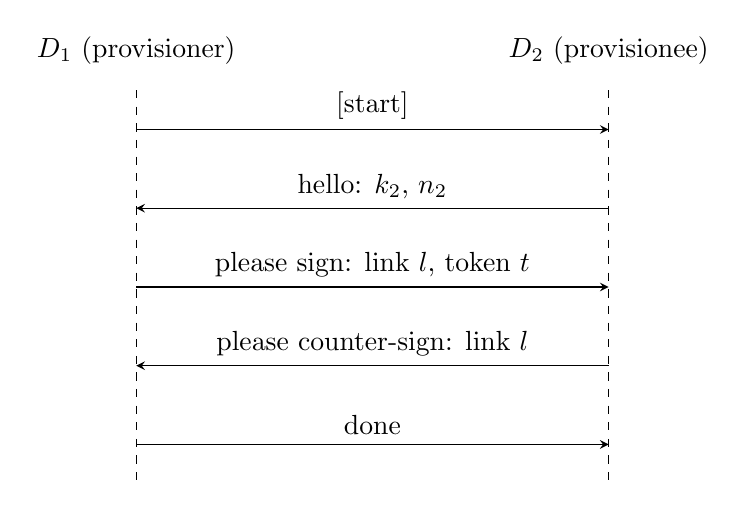
\begin{tikzpicture}[>=stealth]
  \node (d1) at (0,6) {$D_1$ (provisioner)};
  \node (d2) at (6,6) {$D_2$ (provisionee)};

  \draw[->] ($(d1)+(0,-1)$) -- node[above] {[start]} ($(d2)+(0,-1)$);
  \draw[->] ($(d2)+(0,-2)$) -- node[above] {hello: $k_2$, $n_2$} ($(d1)+(0,-2)$);
  \draw[->] ($(d1)+(0,-3)$) -- node[above] {please sign: link $l$, token $t$} ($(d2)+(0,-3)$);
  \draw[->] ($(d2)+(0,-4)$) -- node[above] {please counter-sign: link $l$} ($(d1)+(0,-4)$);
  \draw[->] ($(d1)+(0,-5)$) -- node[above] {done} ($(d2)+(0,-5)$);
  
  \draw[dashed] ($(d1)+(0,-.5)$) -- ($(d1)+(0,-5.5)$);
  \draw[dashed] ($(d2)+(0,-.5)$) -- ($(d2)+(0,-5.5)$);
\end{tikzpicture}
\end{center}

The first message, ``start'', is optional and only needed in the case that $s_2$
is entered on device $D_1$. In the ``hello'' message, the provisionee sends its
new key and desired device name over to the provisioner. The provisioner then
makes a sigchain link, $l$, and in the ``please sign'' message, asks the
provisionee to sign it with $k_2$, the new device key. The provisoner also
includes token $t$ so the provisionee can load the user's sigchain from the
server. In the ``please counter-sign'' message, the provisionee returns the
signed link and asks the provisioner sign it a second time with $k_1$, $D_1$'s
device key. Finally, the provisioner can post the new signed sigchain link $l$
to the server, including encryption of the latest PUK for $k_2$ with $l$. Once
the provisionee receives the ``done'' message, it can load the user's PUKs from
the server, and decrypt them with $k_2$.

Though messages between $D_1$ and $D_2$ could use interesting local peer-to-peer
protocols, we employ a simpler, more reliable strategy. The FOKS server proxies
all of these messages. One device sends a message, while the other polls for the
next message in the sequence. Let $s^{*}$ be the session key that was input on
the other device. Both devices encrypt all messages send to the server with the
session key $s^{*}$, using authenticated encryption.

Some researchers~\cite{ncc2019} have suggested using a passphrase-authenticated
key exchange (PAKE) rather than this simple $s_1$ / $s_2$ mechanism. The
observation is that the secret phrases, which users have to type until
smart-phone apps are built, are quite long and could be much shorter with PAKEs.
We considered these constructions but rejected them for FOKS, since we are
concerned the PAKEs can be easily DOSed. That is, the provisionee $D_2$ is not
authenticated to the server since the user hasn't logged in on $D_2$ yet; this
login happens naturally as a result of the provisioning process. Thus, there is
nothing to stop an attacker from targeting a user and entering bad PAKE codes
before the legimiate user can enter the correct code. Such an attack would not
break the integrity of the protocol, but could prevent the user from ever
successfully provisioning.

Note that several of these provisioning sessions can happen concurrently on the
same the server. $D_1$ and $D_2$, with the server's assistance, must separate
their messages from other currently active clients.  They therefore tag each
message in the exchange with the channel identifier $H(s^{*})$, where $H$ is a
one-way function like SHA2. This channel identifier is unguessable for 
any malicious clients who do not know $s^{*}$, and will clearly be unique
across all device pairs.

\subsubsection{\Yubi -to-Device and Device-to-\Yubi }

Most of the protocol in Section~\ref{sec:kex} can be skipped in the case
of either provisioning a regular device (a computer or a phone) with a \yubi ,
or vice versa. No communication needs to bounce off the server, as the device
and the \yubi{} can comunicate directly via the local machine. The crux of 
the protocol, however, remains. For a \yubi{} provisioning a new device,
the device makes the new link, the device signs the link, and the \yubi{} 
countersigns it. Then the device posts the link (and encrypted PUK keys)
to the server. And vice-versa for a device adding a new \yubi . 

\subsection{Teams}
\label{sec:teams}

We covered much of how teams work in Section~\ref{sec:sigchains}, largely by
analogy to users and devices. There are, however, some important differences,
which we cover here in more detail.

\subsubsection{Cross-Server Teams}

As described in Section~\ref{sec:sigchains}, teams are composed of parties
that can span multiple federated servers. A team has a home server, which 
hosts its public keys, encrypted secret keys, sigchain, and Merkle Tree.
An importantly, all the admins and owners --- those who have the ability
to change the team --- must be on the same home server. However, team readers
can join the team from across the Internet.

Because readers can be local or remote, important team protocols, like addition
and removal, must work with more generality, as we cannot assume that the reader
and the team have the same home server. Morever, we cannot assume much
cooperation among independently administered servers under our thread model
(see Section~\ref{sec:threatmodel}).

\subsubsection{Cycle Avoidance}
\label{sec:team-index-range}

One problem in particular the presents itself immediately: potential cycles.
Imagine a simple case, with three hosts $h_1$, $h_2$ and $h_3$, and three teams
on those host, respectively, $t_1$, $t_2$ and $t_3$. If $t_1$ adds $t_2$ as a
reader, $t_2$ adds $t_3$ as a reader, and $t_3$ adds $t_1$ as a reader, there is
now a cycle in the team membership graph. That cycles are bad is not immediately
obvious, but we must consider what happens in a rekey scenario.

Imagine at the start of the sequence, team $t_1$ consists of two owners --- call
then $u$ and $v$ --- and no other members. Team $t_2$ consists of a single owner
$x$, and team $t_3$ consists a single owner $y$. Focus on user $v$, who will
eventually be removed.  At the start $v$ has access to $t_1$'s reader PTK at
generation 1, call it $k^{1}$.  Next, $x$ adds the readers of $t_1$ to $t_2$
as readers. As a result, $v$ gets access via $k_1$ to $t_2$'s reader PTK,
call it $k_2$. Next, user $y$ adds the readers of $t_2$ to $t_3$ as readers,
giving $v$ access to $t_3$'s PTK $k_3^{1}$ transitively via $k_1$ and $k_2$.
Finally, $u$ completes the cycle, adding the readers of $t_3$ to $t_1$ as readers.
Figure~\ref{fig:cycle1} shows this initial configuration. 

\begin{figure}[ht]
    \centering
    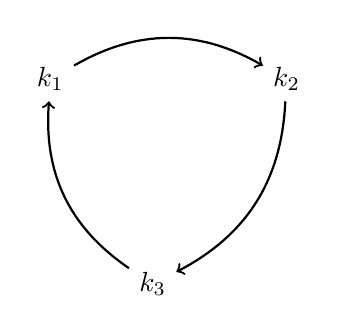
\begin{tikzpicture}[->, thick, auto, node distance=2.5cm]
        \node (k1) at (0,0) {$k_1$};
        \node (k2) at (3,0) {$k_2$};
        \node (k3) at (1.3, -2.598) {$k_3$};
      
        \draw[bend left=30] (k1) to (k2);
        \draw[bend left=30] (k2) to (k3);
        \draw[bend left=30] (k3) to (k1);
      \end{tikzpicture}
    \caption{The initial configuration of teams $t_1$, $t_2$ and $t_3$.
A link from $k$ to $j$ means that knowing $k$ gives one access to $j$, i.e., that $k$ is a reader of $j$.}
    \label{fig:cycle1}
\end{figure}


Everything up until now is working as planned, but now consider what happens when
$u$ removes $v$ from $t_1$. What should happen is that all 3 teams should 
rotate so that $v$ loses access to their most recent reader PTKs. But in practice, this
objective cannot be achieved. Playing out the scenario, $u$ rotates $t_1$'s reader PTK
from $k_1$ to $k_1'$. It encrypts $k_1'$ for $k_1$ so that the remaining 
members can still access old data. It also encrypts $k_1'$ for $t_2$'s most recent reader
PTK, which remains $k_2$. See Figure~\ref{fig:cycle2} for what this new configuration looks like.
One thing to notice immeidately is that any node on the graph is reachable from any other. That is,
if user $v$ knows $k_1$ (which he had access to before $u$ removed him), then he can still
decrypt any other key on the graph, including $k_1'$, which he reach via
$k_1 \rightarrow k_2 \rightarrow k_3 \rightarrow k_1'$. So in a deep sense, the 
rotation has failed. 

\begin{figure}[ht]
    \centering
    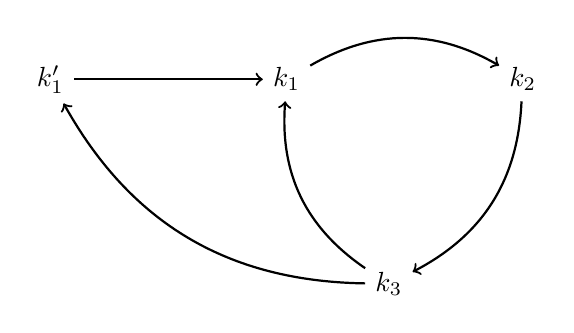
\begin{tikzpicture}[->, thick, auto, node distance=2.5cm]
        \node (k1) at (0,0){$k_1$};
        \node (k2) at (3,0)  {$k_2$};
        \node (k3) at (1.3, -2.598) {$k_3$};
        \node (k12) at (-3, 0) {$k_1'$};
      
        \draw[bend left=30] (k1) to (k2);
        \draw[bend left=30] (k2) to (k3);
        \draw[bend left=30] (k3) to (k1);
        \draw (k12) to (k1);
        \draw[bend left=30] (k3) to (k12);

      \end{tikzpicture}
    \caption{After $u$ removes $v$ from $t_1$ and rotates $t_1$'s reader PTK to $k_1'$.}
    \label{fig:cycle2}
\end{figure}

To continue a few more steps, assume $t_2$ rotates (see Figure~\ref{fig:cycle3}), 
and then $t_3$ rotates (see Figure~\ref{fig:cycle4}).
for the new configuration. The problem remains. Any node in the graph is reachable from any other,
and therefore, $v$ can still access the new PTKs for all teams. We can generalize (without proof)
that there is no ``fixed point'' during this decentralized key rotation process, and that no amount
of rotation will lock $v$ out of the teams. A different system in which $t_1$, $t_2$ and $t_3$
rotated simultaneously might avoid this problem, but we see no robust way for them to do so 
if those teams reside on independent servers.

\begin{figure}[ht]
    \centering
    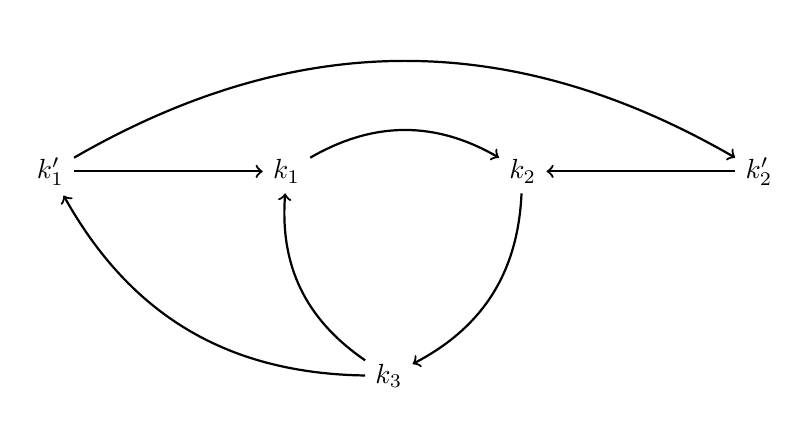
\begin{tikzpicture}[->, thick, auto, node distance=2.5cm]
        \node (k1) at (0,0){$k_1$};
        \node (k2) at (3,0)  {$k_2$};
        \node (k3) at (1.3, -2.598) {$k_3$};
        \node (k12) at (-3, 0) {$k_1'$};
        \node (k22) at (6,0) {$k_2'$};
      
        \draw[bend left=30] (k1) to (k2);
        \draw[bend left=30] (k2) to (k3);
        \draw[bend left=30] (k3) to (k1);
        \draw (k12) to (k1);
        \draw[bend left=30] (k3) to (k12);

        \draw[bend left=30] (k12) to (k22);
        \draw (k22) to (k2);
      \end{tikzpicture}
    \caption{\textit{The Widening Gyre}: After $u$ removes $v$, $t_1$ rotates, then $t_2$ rotates.}
    \label{fig:cycle3}
\end{figure}

\begin{figure}[ht]
    \centering
    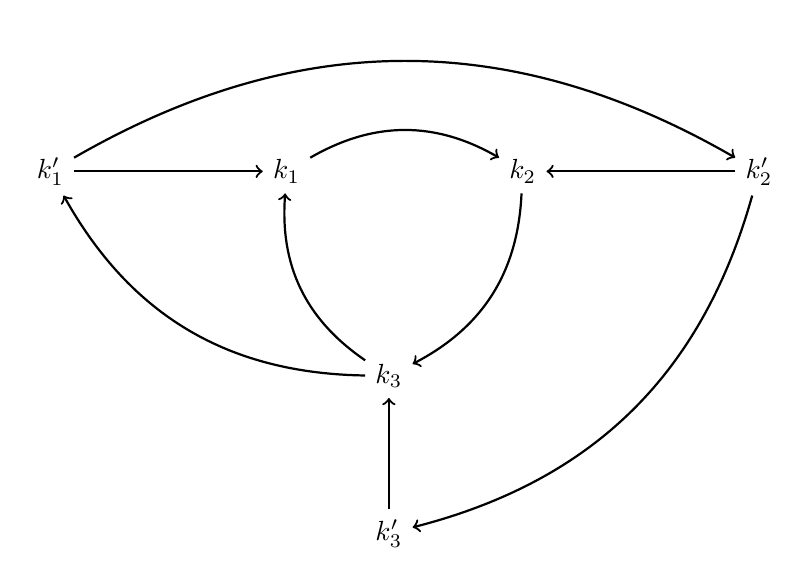
\begin{tikzpicture}[->, thick, auto, node distance=2.5cm]
        \node (k1) at (0,0){$k_1$};
        \node (k2) at (3,0)  {$k_2$};
        \node (k3) at (1.3, -2.598) {$k_3$};
        \node (k12) at (-3, 0) {$k_1'$};
        \node (k22) at (6,0) {$k_2'$};
        \node (k32) at (1.3, -4.598) {$k_3'$};
      
        \draw[bend left=30] (k1) to (k2);
        \draw[bend left=30] (k2) to (k3);
        \draw[bend left=30] (k3) to (k1);
        \draw (k12) to (k1);
        \draw[bend left=30] (k3) to (k12);

        \draw[bend left=30] (k12) to (k22);
        \draw (k22) to (k2);

        \draw (k32) to (k3);
        \draw[bend left=30] (k22) to (k32);

      \end{tikzpicture}
    \caption{\textit{Things Fall Apart}: After $u$ removes $v$, $t_1$ rotates, then $t_2$ rotates, and finally $t_3$ rotates.}
    \label{fig:cycle4}
\end{figure}

The simplest path forward is to disallow cycles in the global team
graph, which seems like a natural constraint. However, enforcing
lack of cycles globally is challenging, and seems to require some
concept of global locks across the internet. To see why, consider
four teams, $t_1$, $t_2$, $t_3$ and $t_4$, on four different servers.
First, $t_1$ adds $t_2$ as a reader, and $t_3$ adds $t_4$ as a reader.
So far so good. If $t_2$ adds $t_3$ as a reader, or $t_4$ adds
$t_1$ as a reader, we still are cycle-free.  But if the two additions
happen roughly simultaneously, a cycle is formed, and there is no easy
way for any of the hosts involves to detect it.

The most blunt and naive solution is for each team to get an ``index'', which
which is simply a natural number. This index cannot change once assigned, and
$t_1$ can only add $t_2$ iff $t_2$'s index is less than $t_1$'s. This simple
rule prevents cycles, but is inflexible and doesn't allow much play in the team
graph as the system evolves. FOKS opts for a slightly more flexible solution of
a similar flavor. Each team gets a ``range'' of possible index values,
representing bounds on where the team's index will eventually settle.  This
range in practice is an interval on the positive rational numbers, of the form
$[a,b)$, where $a,b \in \mathbb{Q^{+}}$. $b$ can take on the special value $\infty$.
A team can always restrict its range but can never expand it. The rule for
addition then becomes that $t_1$ can add $t_2$ iff the lower bound of $t_1$'s
range is greater than the upper bound of $t_2$'s range. The rule guarantees that
whereever $t_1$ and $t_2$'s indices eventually settle, $t_1$'s index is greater
than $t_2$'s.

All teams get the initial default range of $[1,\infty)$. When a team administrator
seeks to add one team to another, she might need to change one or both of the team's
ranges. For instance, take teams $t_1$ and $t_2$, both at the default range $[1,\infty)$.
To add $t_1$ to $t_2$ as a reader, the administrator can reduce $t_1$'s range to $[1, 128)$
and team $t_2$'s range to $[128, \infty)$. Now the property above is upheld,
since $[1,128) < [128, \infty)$.  Note that it still remains possible to add $t_2$ to 
another team or to add another team to $t_1$ by making appropriate range reductions.

\subsubsection{Invitation Sequence}
\label{sec:invitation}

By default, two parties $p$ and $q$ cannot view each other's sigchains, even if on the same
server. But $p$ must be able to read $q$'s sigchain in order to compute its current
PUKs or PTKs if adding $q$ to a team. So a protocol must be invented to allow $p$ and $q$
to exchange information before the actual join process occurs. There are three general
steps: (1) $p$ creates a multi-use invitation token, which $p$ can share with one or
more parties; this invitation exposes the team's name, host and ID to all invitees; 
(2) $q$ ``accepts'' this invitation, thereby granting $p$ access to its sigchain;
and (3) $p$ ``admits`` $q$ into the team.

\paragraph{Invite Tokens}

A team's administrator or owner can create a multi-use invitation token for a team $t$.
First, the administrator creates a team certificate with the fields:

\begin{itemize}[noitemsep]
    \item The team's ID
    \item The team's Host ID
    \item The team's current admin PTK
    \item The current time
    \item The name of the team
    \item The team's index range
\end{itemize}
%
The adminstrator then signs this certificate payload with both the current PTK, 
and also the original PTK, whose hash is the team's ID.  If the PTK hasn't rotated,
then of course only one signature suffices. In totality, the above data and the signatures
are quite large, so we introduce one layer of indirection to make them shorter. 
The administrator posts the signed certificate it's home server, and then formulates
an invitattation as: (1) the hash of the above data; and (2) the host's ID. The
resulting token can look something like this:
%
\begin{verbatim}
    YcarI5JTMAVDHG47cb5l1Pp87COqmK6nzf6h12hchVLMMjlplmjC5dky
    wwnqlOhuakWkAjzO2zJ6BtxrnOxdZV8NyLby2r16MhCvC
\end{verbatim}
% 
Which is small enough to exchange via group text chat.

\paragraph{Accepting Invitations}

Once a party $p$ receives the invitation to team $t$ ($p$ can be a user or a
user acting on behalf of a team), it breaks the token into its two parts, the
host ID and the certificate hash. It maps the host ID to a DNS name (see
Section~\ref{sec:beacon}), and then asks the server for the preimage of the hash
from the invitation. It checks that the preimage hashes correctly, and then
opens the certificate. From here, it checks the signatures described just above.
Note that at this point, $p$ is not a member of the team, so cannot read the
team's sigchain. 

There is therefore an oppoortunity for the team certificate to be partially
forged. $p$ can check that that first PTK corresponds to the team ID, so
therefore knows that whoever generated this certificate was at one time a team
admin.  But that administrator might have been removed from the team. Also, the
name of the team cannot be checked against the Merkle Tree, so the team's name
might be forged. Eventually, once $p$ is admitted into the team, it can check
that these fields are correct, and leave the team if not.  By accepting the
invitation, be it malicious or otherwise, $p$ is primarily giving access to
reading its sighcain. It must decide whether or not this is a good idea on the
basis of who sent the team invitation in the first place. This problem can
recursively be solved in FOKS, by a different team, or by trusted channel on a
different platform, like a secure team chat.

If $p$ decides to accept this invitation, there are four subcases to consider:

\begin{enumerate}
\item $p$ is a user, and $p$ and $t$ are on the same server.
%
Here, the user $p$
instructs her home server to allow the owners and administrators of $t$ to allow
access to her sigchain. The server makes a quick note in the database to honor
future accesses. Then $p$ writes a link to its Team Membership Chain (see Section~\ref{sec:subchains}) 
saying it accepted an invitation to team $t$.
\label{case:user-user-local}

\item $p$ is a user, and $p$ and $t$ are on different servers.
%
User $p$ contacts its home server and asks that it assue a new 
``remote view permission token'' for the administratos and owners of $t$.
The server sends back this token. $p$ encrypts this token with the PTK
it received in the team's certifcate, and then posts this encryption to
$t$'s home server. Note that $p$ isn't trusting the server's administrators 
here, so does not send this token in plaintext. As with the above case,
$p$ writes a link to its Team Membership Chain saying it accepted an invitation
to $t$. It also informs $t$'s server that it has accepted the invitation.
\label{case:user-user-remote}

\item $p$ is a team, and $p$ and $t$ are on the same server. 
% 
The actor here is an an administrator or owner of team $p$. He firsts does a
cycle check, checking that the index range of $p$ is less than that of $t$.
The server would reject the addition of $p$ otherwise. The admin/owner now
operates analogously to Case~\ref{case:user-user-local}.  First, he
instructs the server to allow the admins of $t$ to read $p$'s sigchain.
Then, he posts a link to $p$'s Team Membership Chain saying that it has
accepted an invitation to $t$.
\label{case:team-team-local}
    
\item $p$ is a team, and $p$ and $t$ are on different servers.
%
This case is a hybrid of Cases~\ref{case:user-user-remote} and~\ref{case:team-team-local}.
As in Case~\ref{case:team-team-local}, the actor first performs a cycle check.
As in Case~\ref{case:user-user-remote}, the actor makes a new review view token
for $p$ and posts it to $t$'s home server. Then it writes a link to $p$'s
Team Membership Chain as above.
\label{case:team-team-remote}

\end{enumerate}

\paragraph{Admitting into Teams}

For a given team $t$, the owners and administrators see an inbox of pending
accepted invitations. For each of these, the administratos makes a yes/no
decision as to whether the team can be admitted into the team, and also what
it's role should be in the new team. Recall some restrictions on these roles: 
(1) remote parties can only be readers; and (2) administrators cannot add new
members to teams as owners. In any of the four subcases above, the administrator
gets the necessary access to play the accepted party's sigchain; as such,
he can put their latest PUK or PTK into the sigchain, and can encrypt
$t$'s latest PTK for that PUK or PTK.

Once the party is admitted into the team, it can sign a statement with its PTK
or PUK to play the team's sigchain. When it does that for the first time, it
updates its Team Memership Chain to show that the accepted invite transitioned
to an official admittance. 

\subsubsection{Team Key Rotations}
\label{sec:clkr}

PTKs must be rotated in two important cases: (1) when a party is removed from a team; and (2)
when a member rotates their PTK or PUK. The first case is straightforward, and happens
when the administrator performs the removal. In such a case, the adminstrator (or owner)
posts a new link to the team's sigchain with the role of \none{} for the affected party.
The link also contains the new PTKs for the team. The administator also includes
new encryption of these PTKs for the remaining members of the team.

The trickier case is the second, since the rotations happen asynchronously. Say
that user $u$ is a member of team $t_1$ which is in turn a member of team $t_2$.
Now say user $u$ revokes a device, mayb because it was lost or stolen. Upon
revocation, his PUKs will rotate. Eventually the PTKs for $t_1$ must rotate,
which will eventually trigger a rotation for $t_2$. But there are several
reasons these rotates might not be immediate. Perhaps all the relevant
adminstrators (who are authorized to perform the rotations) are offline. Or
maybe $t_1$ or $t_2$ is hosted on a different server which is currently offline
for maintenance. Since it is clear that some cascading team key rotations must
be done asynchronously, we simplify the FOKS systems by having \textit{all} team
rotations happen asynchronously along the same code paths.

Every FOKS clients polls all reachable teams in a background loop. It starts 
with teams in the user's team membership chain, then recursively loads all teams
and their associated membership chains, in a breadth-first manner.  For each
team encountered where the user can act as an administrator, either directly or
via a team, it checks that all PTKs and PUKs in the team chain are up-to-date.
If it finds one that is behind for any member, it will rotate necessary PTKs so
they are encrypted for the member's latest keys. Rekeying starts with teams
that have the lowest index ranges, and moves upwards, so that cascaing rekeys
happen in the right order.

If there are multiple administrators or owners for teams, there is no explicit
coordination. Rather, they in effect race to rekey the same teams.  However, the
FOKS client adds randomness into the traversal order where possible, and
randomness into the timing, so chances of collisions are low. If they do happen,
the loser of the race will fail to update the team chain (as enforced by the
server), will reload the team, and then see it no longer needs to rekey.

Note the importance of the Team Membership Chains in this protocol. The
users should not trust the servers to faithfully recount to them which
teams they are members of; if they did, dishonest servers could silently
supress team rotation through omission. Instead, the Merkle Tree and sigchain
append-only properties give users guarantees that servers aren't tampering
1Gwith their view of team memberships.

Also note that to perform this ongoing key rotation process, all team
administrators need ongoing access to the sigchain of team's members. Thus, the
access tokens and permissions exchanged as part of the team invitation process
(see Section~\ref{sec:invitation}) persist in the team as long as mebmers
remain.

\subsubsection{Removal Keys}
\label{sec:removal-keys}

When users are removed from teams, they should no longer be able to load the team's
sigchain. But what's to stop a server from falselyclaiming the user was removed, thereby 
preventing the user from rotating the team as described in Section~\ref{sec:clkr}?
We here discuss ``Team Removal Keys'', which allow a team administrator to prove
to a removed team member that they were legitimately removed, rather than falsely
removed as a malicious server might claim.

Recall from Section~\ref{sec:sigchains} that when administrator add members to
teams, they include for each member a commitment to a ``team removal key''. Here
is where this mechanism comes into play. The team removal key is a 32-byte
random value, generated anew for each member added to the team. When adding
member $p$ to the team, the administrator encrypts this removal key for the
other administrators for the team, and also for $p$'s PTK (or PUK, depending if
$p$ is a user or a team). The administrator puts both ciphertexts to the server,
and writes a commitment to this key into the sigchain link. When $p$ loads the 
team and plays the sigchain, it writes down this commitment to a local database.

Later, when an administator removes $p$ from the team, $p$ will fail to load
new chainlinks from the team, though it should still keep existing chainlinks
in its cache. It can now demand ``proof'' from the server that its removal
was legitimate. If indeed it was, the server will send down the ciphertext
computed at addition time, and $p$ can decrypt it. It can check this key
against the commitment in the team chain that it has written to a local database.
It can further check that the administrator MAC'ed a statement with this
key, stating that $p$ was removed from the team and the time of the removal.
If the decryption of the key fails, or if the key does not match the commitment
in the team chain, or if the MAC of the removal statement fails, the software
can post a warning to the user's client, saying that it suspects some form
of server tampering.

Members $p$'s team removal key is not rotated when $p$ rotates their PTK or PUK;
nor is it rotated when the admins or owners of the team change. Lack of rotation
opens the window for an attack; a malicious server collaborating with an
attacker who gains access to a stolen device can recover the team removal key
and make a false statement that $p$ has been removed from the team. Though it is 
possible to replace and rotate team removal keys when member PTKs or PUKs change,
such rotations create new challenges. If members fall behind the latest
team removal keys and then are removed, they will have no commitment to 
compare the new removal key against, preventing the protocol from workking.
We believe the correct trade-off is to keep the original team removal key
despite other rotations.

\subsection{Beacon Server}
\label{sec:beacon}

When a user is discovering a new server, there are two types of lookups that are
required: (1) mapping from a standard DNS name to a the server's ID; and (2)
going the other direction. The first direction is straightforward.  The user's
client makes a TLS connection to the server's name, and retrieves a hostchain.
The client uses the standard root CAs to verify that the server's certificate 
matches its DNS name. The returned hostchain is rooted in the server's
initial public key, and potentially contains several key rotations. The most
recent key must sign the host's DNS name, allowing the client to verify the
correspondence between the two. 

Once the server makes an initial mapping of a domain name like
\texttt{example.com} to a host ID $h$, the user's client writes it down in its
local database, and it is ``pinned'' going forward. The server can change to a
new hostname \texttt{example.io} through the normal operation of the
hostchain. But the original hostname should never be reused by a different
server.

Sometimes clients need to perform the opposite mapping, from host ID
to DNS name. Users are allowed to refer to servers by their host ID
and might choose to do so if they have reason to mistrust the 
root CAs~\cite{diginotar}. While more sophisticated solutions are possible
(like DHTs~\cite{chord} and blockchains~\cite{bitcoin}), FOKS opts for a simple
solution for now. We host a single ``beacon'' server, which is a simple
server that maps host IDs to DNS names. Clients take these mappings
with a grain of salt but can verify them via the hostchain protocols
described above.



\subsection{Privacy}
\label{sec:sigchain-viz}

Previous systems like Keybase~\cite{keybase} espoused a notion of transparency
regarding a user's identity and devices. Any user $u$ is free to load the 
sigchain of any other user $v$ on the system, and can learn how many devices $v$
has, when those devices were added to $v$'s sigchain, and the names of these
devices. Howver, team membership was private, so $u$ could only load team $t$'s
sigchain, or learn team $t$'s name, if $u$ is on team $t$.  Zoom's
system~\cite{zoom-privacy} is derived from Keybase's, by because it caters to
enterprise settings, opts for more privacy, obscuring most deatils about user's
identities.

As described above, FOKS takes, by default, the more privacy-respecting
approach, similar to that of Zoom's system. User $u$ can load $v$'s sigchain
only if $u$ allows it. The team invitation flow~\ref{sec:invitation} is an
example of how $v$ shares a view of his sigchain only as required.  However,
server administrators can configure their server in FOKS to have different
policies.  A server, for instance, can allow all logged-in users to see each
other without need for explicit permissions. A complementary policy might be
that $v$ can always directly add $u$ to a team, and if $u$ is unhappy with this
situation, he can leave. This configuration might work well for a
company-specific server.

Another important privacy feature is how device names are handled. As
described in Section~\ref{sec:sigchains}, users do not write 
device names directly into sigchain links.  Instead, when provisioning
a device name $n$, the user picks a random 32-byte value $r$, and publishes
$Hmac(n, r)$ into the sigchain. On playback, the server returns $r$ and $n$, 
so the user can check it's the same value as intended. If the user later
regrets the choice of $n$, the server can throw $n$ and $r$ away while
still allowing playback of the sigchain.


\section{Cryptographic Design}
\label{sec:crypto}

Here we describe the important cryptographic decisions at play in the FOKS
system.  For the most part, our bias is toward simplicity and boring,
failure-proof cryptography.  For instance, as decribed in
Section~\ref{sec:merkle}, we use a vanilla collision-resistant hash function to
hide tree locations, rather than the slightly more exotic pseudo-random function
approach. The emphasis throughout is on tried-and-true cryptography that will
prove as robust as possible to misuse through software bugs.

\subsection{The Snowpack Domain-Specific Language}

One of the biggest risks in a system like FOKS is signature malleability
due to issues like permitting non-canonical encodings~\cite{conf/crypto/Bleichenbacher98,bip66}, 
lack of clear domain separation~\cite{ncc2019,cryptoeprint:2020/241}, 
or undefined behavior due to parsing and encoding bugs~\cite{heartbleed2014durumeric}.

To address these threats, and at the same time to provide an convenient language for 
defining RPC protocols, we introduce the Snowpack Language~\cite{snowpack}, which is influenced
by protobufs~\cite{protobuf}, Framed Msgpack-RPC as used in Keybase~\cite{keybase}
and Cap'n Proto~\cite{capnproto}. A further property we insist upon is support
for backwards and forwards compatibility. Since FOKS is a federated system, we have 
no expectations that upgrades will happen in lockstep. The protocol itself must behave
well in any number of partially-upgraded configurations.

\subsubsection{Structures}
\label{sec:snowpack-structures}

By way of example, see Figure~\ref{fig:group-change} for the definition of a sigchain link both for teams
and users in the Snowpack language. Any constant of the form \texttt{@1} or \texttt{@0x8fbf37f586b0bc6e}
is meant to be \textit{immutable}. Once written down in the protocol, it should never change. For instance,
look at the first field in the structure: \texttt{chainer @0 : HidingChainer;}. The \texttt{@0} indicates that this
field will take the 0th slot in the encoded version of the structure. Future editors of this file must
never introduce a new field at slot 0 with a different type, as that would cause old clients to fail
in decoding. All new fields should be added at the end of the structure. Old clients will ignore fields
from the future that they do not know how to decode. Similarly, it is allowable to delete a field.
Software with older version of the protocol will get 0 values for the deleted fields. In the Go language,
this means \texttt{0} for integers, empty strings for strings, empty slices for lists, and nil 
pointers for optional fields. Of course new clients must consider the impact on older clients to 
leave 0-ed fields, but the protocol layer itself does not introduce a failure here.

\begin{figure}[ht]
  \centering
\begin{verbatim}
  struct GroupChange @0x8fbf37f586b0bc6e {
    chainer @0 : HidingChainer;
    entity @1 : FQEntity;
    signer @2 : GroupChangeSigner;
    changes @3 : List(MemberRole);
    sharedKeys @5 : List(SharedKey);
    metadata @6 : List(ChangeMetadata);
}
\end{verbatim}
\caption{A sigchain link in the Snowpack language.}
\label{fig:group-change}
\end{figure}

Structures like \texttt{GroupChange} from Figure~\ref{fig:group-change} are
encoded as JSON-style arrays on the wire, with fields written to slots as
directed by their \texttt{@i}-style positions. Elided fields are written down as
\texttt{null} values. Before going out to the wire, the JSON-style arrays are
encoded with the Msgpack~\cite{msgpack} encoding format. Where two possible
encodings are possible (e.g., the number \texttt{0x2} can be encoded as
\texttt{0x2} or \texttt{0xcd 0x00 0x02}), the shorter encoding is mandated. Note
that field names (like \texttt{chainer} above) are not sent over the wire, but
are available on either end as human-readable references to fields. Thus, it is
permitted to rename a field as long as its type doesn't change. We note that
serializing using JSON-style dictionaries seems error-prone, since keys can
repeat or be ordered in different ways. Snowpack's slot-oriented encoding aims
to avoid these styles of ambiguities and to minimize encoding sizes. At the same
time, development tools can decode encoded messages without reference to
protocol specification files.

\subsubsection{Domain Separation}

In the definition of the \texttt{GroupChange} structure from
Figure~\ref{fig:group-change}, note the 64-bit integer
\texttt{@0x8fbf3...}. This is a randomly-generated number that serves as
a \textit{domain separator}. We refer to it below as unique type identifier
(UTID). Though domain specifiers are optional in the Snowpack language, when a
structure provides it, the snowpack compiler fills in five possible
cryptographic operations for the structure:
%
\begin{itemize}

  \item \texttt{PrefixedHash}(\textit{obj}): The object's UTID is big-endian encoded, then
  prepended to the object's binary Msgpack encoding. The hash of the combined message is returned.

  \item \texttt{Hmac}(\textit{obj}, \textit{key}): As above, a mesasge is formed out of the object's UTID
  concatenated with the encoding of the object itself. The combined message is the message input
  to the MAC function, and the key is passed through as the key.

  \item \texttt{SealIntoSecretBox}(\textit{obj}, \textit{nonce}, \textit{key}): The object's UTID is
  encoded and conctacted with the supplied \textit{nonce}. The new value is then used as the nonce
  passed into the encryption algorithm, along with the encoding of \textit{obj} and the supplied \textit{key}.

  \item \texttt{Sign}(\textit{obj}, \textit{key}): The object's UTID is prepended to an encoding
  of \textit{obj}; the combined message is then used as the message input, passed along to the 
  signature algorithm along with the supplied \textit{key}.

\end{itemize}
%
%
Public key encryption calls into \texttt{SealIntoSecretBox} with a random session key, so therefore uses the same
domain separation mechanism. Inverse operations for \texttt{Hmac}, \texttt{SealIntoSecretBox} and \texttt{Sign}
are also provided; they similarly supply UTIDs where necessary to ensure that verification and decryption
succeed.

The programmer must supply their own tooling to generate these UTIDs. Simple CLI tools or 
editor plugins suffice. However, FOKS provides two mechanisms to guararntee they remain unique
across the project. At compile-time, a simple tool examines all input files to guarantee that
no UTID contant appears twice. And at runtime, the compiler provides a list of all UTID constants
compiled from the protocol input files. The program fails an assertion if it sees any repeats.

\subsubsection{Variants}

We have seen Snowpack structures in Section~\ref{sec:snowpack-structures}. Another important
data type is the \textit{variant}, also known as a descriminated union. Figure~\ref{fig:link-inner}
shows an example from FOKS. The enumerated type \texttt{LinkType} has two possible values:
\texttt{GroupChange} for main chains, and \texttt{Generic} for subchains like team membership chains
and user settings chains. Based on the switch value, the enumerated type takes the form of 
a \texttt{GroupChange} or \texttt{GenericLink} object. Variants have many of the same restrictions
as structures: fields specified with `@i'-style slots should never be repurposed, though they 
can be dropped; also, new type possibilites can be added without breaking the protocol.

\begin{figure}[ht]
  \centering
  \begin{verbatim}
    variant LinkInner switch (t : LinkType) @0xacf9066572a9e7de {
      case GroupChange @0 : GroupChange;
      case Generic @1 : GenericLink;
    }\end{verbatim}
  \caption{A variant in the Snowpack language.}
  \label{fig:link-inner}
\end{figure}

\subsection{Cryptographic Primitives}
\label{sec:cryptography}

We have tried as much as possible to make boring, unopinionated cryptographic
decisions.

\subsubsection{Hashing, MAC'ing and Symmetric Encryption}

Throughout the system, hashing uses SHA512 truncated to 256 bits~\cite{rfc6234}.
Message authentication codes are with HMAC~\cite{rfc2104} over SHA512/256. HMAC
is used for MAC'ing but also for commitments, and in general, any context where
a pair of items are hashed together (one being the ``key'' and the other being
the ``data''). Authenticated symmetric encryption uses Salsa20/Poly1305 as
implemented by the NaCl~\cite{nacl} library. Sals20 has a 24-byte nonce field,
which is often handy when combining with our domain separation strategy with
other authenticated data. We throughout refer to encrypting with Salsa20 as
\texttt{secretBox}'ing, as per the library's conventions.

\subsubsection{Signatures and Post-Quantum Encryption}

For signing, we use EdDSA with the Ed25519 curve~\cite{eddsa}.  Public-key
encryption is a hybrid of Diffie-Hellman over
Curve25519~\cite{cryptoeprint:2011:141} and MLKEM~\cite{nist-fips-203} using a
construction similar to X-Wing~\cite{xwing}, but with a different binary
encoding format and constants. Thus, in practice, all device keys, PUKs,
PTKs, and so on are not a single keypair, but rather a triple: an EdDSA 
keypair, a Curve25519 keypair, and an MLKEM keypair. Wherever public keys
are introduced, an EdDSA signature over the Curve25519 and MLKEM public keys
is produced to bind them together.

The exact derivation of the hybrid encryption secret key is specified in 
Snowpack, using the structure shown in Figure~\ref{fig:xwing}. Hash inputs are:
the domain separator (UTID); a version number; the shared key exchanged via KEM;
the shared Diffie-Hellman key; the receiver's public keys; and the sender's
public DH key. Though everywhere in the project we use SHA512/256, here we 
use SHA3 to follow the spirit of the X-wing specification.

\begin{figure}[ht]
  \centering
  \begin{verbatim}
struct HybridSecretKeySHA3Payload @0x8a9e327647262289 {
    version @0 : BoxHybridVersion;
    pqKemKey @1 : KemSharedKey;
    dhSharedKey @2 : DHSharedKey; 
    rcvr @3 : HEPK; // Hybrid Encryption Public Key = DH + KEM Public keys
    sndr @4 : DHPublicKey;
}
  \end{verbatim}
  \caption{Hybrid encryption secret key derivation in the Snowpack language.}
  \label{fig:xwing}
\end{figure}

\subsubsection{Key Derivation}
\label{sec:xwing-key-derivation}

As described just above, each public key in FOKS actually consists of three keypairs. However,
a single 32-byte secret seed suffices to generate all three, which simplifies secret key
management and backup keys.  The key derivation system again uses the Snowpack specification
system and simple HMAC-based key derivation. Figure~\ref{fig:key-derivation} shows the 
Snowpack structures and variants used. The derived key is the HMAC of the \texttt{KeyDerivation} object
with the secret 32-byte seed as the key.

\begin{figure}[ht]
  \centering
  \begin{verbatim}
enum KeyDerivationType {
    // Core types
    Signing @0;
    DH @1;
    SecretBoxKey @2;
    MLKEM @4;
    AppKey @5; // Used for different higher-level applications, like KV Store
}

enum AppKeyDerivationType {
    Enum @0;
    String @1;
}

enum AppKeyEnum {
    KVStore @0;
}

variant KeyDerivation switch (t: KeyDerivationType) @0xd35cdcc95caef674 {
    case MLKEM @4: Uint; // need 2 32-byte values to get a 64-byte seed
    default: void;
}
\end{verbatim}
  \caption{Structures and variants used in key derivation.}
  \label{fig:key-derivation}
\end{figure}

For example, to make a new PTK, the team adminstrator picks a random 32-byte
seed value.  Whenever the PTK is used in a symmetric context (like for
encrypting older PTKs), the key derivation uses \texttt{KeyDerivationType =
SecretBoxKey} as an HMAC input.  Similarly for using the PTK as a signing key.
All derived keys are also 32-bytes with the exception of the ML-KEM key, which
needs 64-bytes. The two halfs of this derived key are generated with the same
mechanism, but using \texttt{MLKEM=0} and \texttt{MLKEM=1} in the
\texttt{KeyDervitation} object as the HMAC input.

\subsubsection{\Yubis}

FOKS supports hardware keys like \yubi{} that support the Personal Identity
Verification~\cite{nist-sp-800-73-5} (PIV) standard.  This standard allows the
device to perform public key cryptopgrahic operations, like ECDSA and
Diffie-Hellman over the p256 elliptic curve~\cite{nist-fips-186-3}. Though we
have chosen the Ed25519 and Curve25519 curves for use everywhere, we now need to
accommodate another curve to fit the PIV standard. Too much ``agility'' has
proven problematic for other systems~\cite{jwt-none}, and we would like to avoid
it as much as possible with FOKS, but we make an exception here for a popular
hardware standard.

The bigger issue with \yubis{} is: what do to about post-quantum security?  To
date, we have not seen a wide release of an algorithm like ML-KEM to hardware
devices, and even if so, we'd like to support older, widely-deployed hardware. 

Since there are no perfect solutions here, we have designed a PQ-secure system
around existing PIVs as follows:

\begin{enumerate}
  \item Extract a "secret" from the PIV module: pick an unused ``retired key management'' slot
  (0x82-0x95), and compute $g^{x^2}$ via the ECDH algorithm. Use this value as the seed
  to create a new ML-KEM keypair. Compute ML-KEM on user's computer after extracting the secret
  and deriving the keys.
  \label{step:pq-secret}

  \item Select a different retired key management slot to use for classical ECDH over curve p256.
  Compute ECDH as usually using the \yubi's hardware.

  \item  Combine the secret keys from the previous two steps using the X-wing-style
  derivation scheme from Section~\ref{sec:xwing-key-derivation}.
\end{enumerate}

An important property of this system is that all of the relevant key material
lives on the \yubi ; none lives on the user's computer. The \yubi is all the
user needs to recover important secrets, even if the computer is lost or suffers
data loss. Further, this system is no less secure than an encryption scheme
without PQ-security, as the classical ECDH computation still happens on the
\yubi{} as normal. That is, we are not forcing the user to choose between PQ and
hardware security.  However, this scheme has an important shortcoming. If the
user later reuses the key management slot in Step~\ref{step:pq-secret} for a
different purpose, and exports the public key $g^x$ from the device, the scheme
is no longer PQ-secure.  A quantum computer could recover $x$ from $g^x$ and
then derive the ML-KEM secret key.  This shortcoming makes us long for better
hardware support for ML-KEM.  However, a mitigating factor here is that PIV is
an infrequently-used standard (and for instance is way less popular than FIDO2).
There are few competing applications using these features and key slots.

\subsubsection{High-Entropy Secret Phrase}
\label{sec:hesp}

For backup device keys (which FOKS users can write on pieces of paper), and 
exchanging provisioning secrets betwewen two computers, FOKS uses a simple
encoding scheme called the ``high-entropy secret phrase''. The pattern is 
a series of random words, each separated by a random number. All
words are chose from the BIP39 wordlist~\cite{bip39}. The exact
parameters depend on the application, and are shown in Table~\ref{tab:hesp-params}.

\begin{table}[ht]
  \centering
  \begin{tabular}{|c|c|c|c|c|c|}
    \hline Application & \# of Words & \# of Numbers & Number Range & Entropy \\
    \hline
    \hline
    Provisioning & 7 & 6 & $[0,2^8-1]$ & $7\cdot 11 + 6\cdot 8 = 125$ \\
    \hline
    Backup Device Key & 8 & 7 & $[0,2^{13}-1]$ & $8\cdot 11 + 7\cdot 13 = 179$ \\
    \hline
  \end{tabular}
  \caption{Parameters for high-entropy secret phrases.}
  \label{tab:hesp-params}
\end{table}


\subsection{Secret Key Management}

Secret keys derive from 32-byte seeds, which never leave the device they are created
on (with the possible exception of backup keys, which are written down on paper).
We discuss here how the FOKS client stores these secret seeds persistently. 

\subsubsection{Secure Enclaves}

Where possible, FOKS uses OS-specific secure enclaves. This is the simple case.
FOKS stores the actual 32-byte seeds in a FOKS-specific keyring file in the user's 
home directory. For each seed, FOKS picks a random 32-byte key to encrypt with, and,
if possible, stores that 32-byte key in the user's OS keyring. 

\subsubsection{Passphrase-based Management}

Though it's not encouragd, FOKS does offer a passphrased-based protection mechanism
for secret key seeds. As above, each secret seed gets its own secret-key wrapping 
material wrapping key (SKMWK). But instead of storing the SKMWKs in the OS keystore,
they are encrypted with a key derived from the user's passphrase. We have important 
design considerations for this system that make it quite complex:

\begin{enumerate}

\item If the user has two computers, $A$ and $B$, and the user changes his passphrase on A, when B comes online
 with the old passphrase, it has to decrypt with the new passphrase.

\item Keys encryped for old passphrases need to eventually be migrated to the new passphrase, so that if
an attacker gets the old passphrase and all server data, they still can't decrypt the key.  Of course
this is only possible if that computer $B$ comes back online after the change, but assuming that
the property should hold.

\item Passphrase recovery: to change the passphrase and recover keys, it is sufficient to know the latest PUK.
 Thus, having a backup paper key or a backup \yubi{} should suffice to ``recover'' a passphrase
 and to allow the user to change it without knowing the old passphrase.

\item As with passphrases, if the PUK is updated, all machines with passphrase-encrypted keys
  should eventually rotate (when they come online) so that they cannot be decrypted with an old PUK.

\end{enumerate}

\label{sec:passphrase}

\newcommand{\secretBox}[2]{\textsf{secretBox}(#1, #2)}
\newcommand{\dhbox}[3]{\textsf{dhBox}(#1, #2, #3)}
\newcommand{\pk}[1]{\textsf{publicKey}(#1)}
\newcommand{\sk}[1]{\textsf{secretKey}(#1)}

We describe the process through a small example: two rotations, one due to a PUK rotation,
and one due to a passphrase change. The net result is three different configurations
(the original, and the two following rotations). The general idea is that we have a new ``session''
key at every update, which is symmetrically encrypts the SKMWKs. The session key gets encrypted
twice: once for a key derived from the current passphrase, and one for the user's PUK. This
allows recovery of the SKMWKs with either the passphrase or the PUK:
%
  \begin{center}
  \begin{tabular}{|c|c|c|c|}
    \hline
     Key & Epoch 0 & Epoch 1 & Epoch 2 \\
     \hline
     \hline
      SKMWK & $r_0$ & $r_1$ & $r_2$ \\
      Session Key & $s_0$ & $s_1$ & $s_2$ \\
      Ephemeral DH Key & $t_0$ & $t_1$ & $t_2$ \\
      Passphrase & $p_0$ & $p_0$ & $p_1$ \\
      PUK & $u_0$ & $u_1$ & $u_1$ \\
     \hline
  \end{tabular}
\end{center}
%
At Epoch 0, we have the initial configuration, which consists of the following three encryptions:
%
\begin{align*}
e_0 &= \secretBox{r_0}{s_0} \\
f_0 &= \dhbox{s_0}{\pk{p_0}}{\sk{t_0}}, \pk{t_0} \\
g_0 &= \secretBox{[s_0,\pk{p_0}]}{u_0} \\
\end{align*}
%
$e_0$ is the encryption of the SKMWK $r_0$ for the session key $s_0$.  $f_0$ is the encryption 
of the session key for the user's current passphrase, $p_0$. To derive $\sk{p_0}$, we employ
a simple stretching algorithm and interpret the result as a Curve25519 secret key; then we
derive $\pk{p_0}$ from the secret key as usual. Finally, $g_0$ is the encryption of the session
key $s_0$ for the user's current PUK. We include $\pk{p_0}$ in the plaintext for reasons
we will see shortly. After the client creates encryptions $e_0$, $f_0$, and $g_0$, it sends them
up to the server, for later user on this and other devices.

At Epoch 1, we have the passphrase stationary at $p_0$  but the user's PUK is rotated from $u_0$ to $u_1$.
We will make a SKMWK $r_1$ and a new session key $s_1$. $s_1$ will be encrypted for the user's
new PUK and for the user's existing passphrase. This user might not have input their
passphrase on this machine, and it would annoy the user to prompt for it for a seemingly
unrelated operation. For this reason, we included $\pk{p_0}$ in the plaintext of $g_0$, which
the user can decrypt with access to the old PUK $u_0$. The new encryptions are then:
%
\begin{align*}
e_1 &= \secretBox{[r_0,r_1]}{s_1} \\
f_1 &= \dhbox{s_1}{\pk{p_0}}{\sk{t_1}}, \pk{t_1} \\
g_1 &= \secretBox{[s_1,\pk{p_0}]}{u_1} \\
\end{align*}

In the next epoch, the user changes their passphrase from $p_0$ to $p_1$, and the PUK remains
at $u_1$. The new encryptions are:
%
\begin{align*}
e_2 &= \secretBox{[r_0,r_1,r_2]}{s_2} \\
f_2 &= \dhbox{s_2}{\pk{p_1}}{\sk{t_2}}, \pk{t_2} \\
g_2 &= \secretBox{[s_2,\pk{p_1}]}{u_1} \\
\end{align*}
%
And so on. It might seem at first that there is an unnecssary layer of indirection with using
SKMWKs $r_i$'s and session keys $s_i$'s. To see why it's required, consider the case of a 
device active around passphrase generation $p_0$, but then turned off for a long time,
only to come back online at a much later passphrase generation, say $p_9$. At this point,
the user has forgotten passphrae $p_0$ and is only expected to know $p_9$. When they try
to unlock secret key materials on this hitherto-mothballed device, they will enter passphrase
$p_9$. The scheme is robust to this scenario. The device pulls $f_9$ down from the server
and derives $\sk{p_9}$ from $p_9$. It can then decrypt $f_9$ and recover the session key $s_9$.
Then, it pulls $e_9$ down from the server, and uses it to recover all historical $r_i$'s, including
$r_0$. With $r_0$, it can decrypt the device's secret key material, encrypted ages ago. After so doing, it discards
the encryption with $r_0$ and then upgrades to an encryption with $r_9$. This way, going forward,
if an attacker steals the device and learns the old passphrase $p_0$, she cannot recover
the secret key material. Decrypting the secret key material requires $r_9$, which only
can be decrypted with the latest passphrase ($p_9$) or the latest PUK.






\section{Applications}

The goal of the FOKS system is primarily: for a user or a group of users to
agree upon a sequence of cryptographic keys so they can perform authenticated,
end-to-end encryption of arbitrary data. As a secondary goal, the system
exposes a set of authorized signing keys to sign on behalf of the group,
so that changes can be properly attributed. From here, we can build
any number of applications. 

For instance, one can imagine an MLS system for group messaging~\cite{MLS} where
the chat keys are the cryptographic combination (via something like HMAC or
SHA3) of: (1) the root of the MLS ratchet tree; and (2) the most current PTKs
available for the FOKS group. In this way, one can simultaneously achieve
Signal-style forward secrecy and FOKS-style team and device management. 

For our first FOKS prototypes, we have focused instead of two important applications:
first, at the foundational level, a simple key-value store. Members of the team
can put and get key-value pairs to the FOKS server. Keys and values are encrypted
with authenticated encryption agains the team's PTKs. A second application, built
atop the first, is an end-to-end encrypted Git server, that is compatiable with
legacy Git clients. We describe them both below.

\subsection{The FOKS Key-Value Store}

The FOKS Key-value (KV) store is an end-to-end encrypted key-value store, with 
a hierchical namespace, local to each party on the system. One can store a value
to any key of the form `/a/b/c'; the value can be a few bytes long, or many gigabytes.
The system provides simple \textit{put} and \textit{get} operations, but also
operations on the namespace, like listing, moving, and deletion of directories. That is,
one can perform an operation like \texttt{mv /a/b /foo} in roughly O(1) time, without
individually mofidying each of the entries stored under \texttt{/a/b}. Symlinks are also 
allowed. Though the system has some important Unix-style file system behaviors,
it does not implement full POSIX~\cite{posix-2017} semantics.

When a user puts a key-value pair into the store, it does so on behalf of a party,
whether themselves personally, or a team. It encrypts the key and value with the latest
PUK or PTK for the acting party. Of course PTKs and PUKs can rotate after the put
happens, so when getting values out of the store, the user might perform a decryption
with an older PTK or PUK, depending on the circumstances. We discuss rotation in
more detail below as we describe the various operations of the system.

\subsubsection{Making a New Directory}

The steps for making a new directory for party $p$ operating at role $r$ are as follows:

\begin{enumerate}
    \item Pick a random 32-byte directory key seed $s$.
    \item Pick a random 16-byte directory ID $i$.
    \item Derive $k$ for application \texttt{KVStore} from $p$'s PTK (or PUK) for role $r$
    \item Encrypt $s$ with key $k$ and nonce $i$.
    \item Post the ciphertext and the the directory ID $i$ to the server.
\end{enumerate}
%
This process creates an new empty directory, floating more or less in space. To link this 
new directory, we first need to walk to the appropriate place in the key tree, and then
modify the parent ``directory entry'' or \textit{dirent} to point to this new directory.
See Section~\ref{sec:walk} for more details on the walking process, but for now, assume
we have found the appropriate parent directory $d$. The client gets the directory key
seeds for the parent directory $d$ either from the server or from the client's local cache,
The client then derivew to keys from this key: a 32-byte HMAC key, and a 32-byte box key.
The client can now form a \textit{dirent} with the fields: (1) the new directory ID $i$; (2)
the parent dirent $d$; (3) the MACs of of the name of directory (the last component of the path),
using the MAC key derived just above; (4) the encryption of this name, using the box key
derived just above; (5) the version number (which starts at 1); (6) the role required to
overwite this entry; and (7) a ``binding MAC'' of the above fields, using the HMAC
key derived for parent directory $d$. The client posts this dirent up the server, and now
the new directory is linked into place. Note, the client can race another client here,
in which case there will be conflict over the triple composed of $d$, the name MAC, and 
the version number. The client that loses the race should download the winning dirent
and potentially try again.

Note that the directory name is MAC'ed and encrypted (using authenticated-encryption) separately.
The fields serve two different purposes: the former allows for lookups, where a client knows
a path and want to discover which directory (or later, file) it points to; the latter allows
for listing, where a client wants to know what is in a directory.

\subsubsection{Walking the Namespace}
\label{sec:walk}

Most operations start with a ``walk'' of the namespace, from the root down to the desired node.
For a path like \textttt{/a/b/c} there are of course three directories along the way,
and three corresponding dirents.  Each party has a designated root directory ID, initialized
by the first user of the KV store for this party. The client can fetch this directory 
with a special RPC, which returns the directory ID and its boxed directory key seeds.
To walk down to \texttt{/a}, the client MAC's the name \texttt{a} with MAC keys 
derived from these seeds, and then queries the server for the dirent in \textttt{/}
with the computer MAC, at the greatest version. This dirent, if found, contains a
```binding MAC```, which cryptographically binds the dirents fields together, as MACed
by the directory's MAC key. The client verifies this MAC, and if it passes, then the next
step in the path is the ``value'' field of the dirent, which contains the directory ID
of \texttt{/a}. This process continues until the leaf is reached.

To reduce latency, clients make heavy use of local caching. As they walk, they write down
which dirents they passed through and which versinos of those dirents that they saw.
At the end of the process, the send up the whole path to the server, asking if any dirent
was stale. If so, the clients repeats parts of the walk to get fresh data. 

Note there is a special ``value'' field for ``tombstones,'' which signify that the 
file at the path was deleted. That value can later be reinsted if a subsequent version
of the dirent replaces the tombstone with a value that points to a directory or file.

A dishonest server can withhold fresh dirent versions, which might mask file
updates, deletions or creations. Future improvements to this design might
include a transparency tree akin to the existing Merkle Trees to force the
server to be honest. The throughput and performance of this tree is a challenge
that we so far have not tackled.

\subsubsection{Creating Small Files}

\subsubsection{Creating Large Files}

\subsubsection{Listing Directories}

\subsubsection{Key Rotations}


\subsection{The FOKS Git Server}

\section{Related Work}

The initial inspiration for FOKS is the SUNDR project~\cite{sundr}, which first
originated the idea of a fork-consistent blockchain of edits facilitated by a
untrusted server.  Like Keybase~\cite{keybase}, FOKS applies this basic
architecture to the problem of key distribution, rather than the data those keys
might secure. Many other projects have influenced FOKS's design, like
CONIKS~\cite{melara2015coniks}, SEEMless~\cite{chase2019seemless}, 
ELEKTRA~\cite{cryptoeprint:2024/107}, Zoom's E2EE system~\cite{zoom_e2e_v4}, 
OPTIKS~\cite{cryptoeprint:2023/1515} and the widespread adoption of Key
Transparency in Signal, WhatsApp and iMessage. The question of federation has
largely been ignored, as these systems all shared the basic architecture of a
single upstream server. 

Projects such as Matrix~\cite{matrix} and Mastodon~\cite{mastadon} have
demonstrated the power of federation in other domains but focus on different
applications, like chat and social media. Various IETF drafts are considering
Key Transparency~\cite{ietf-keytrans-architecture-03} and identity
extensions~\cite{barnes-mimi-identity-arch-02} to Messaging Layer Security
(MLS)~\cite{rfc9420} but so far do not provide a complete solution for the use
case described in this paper.

\section{Conclusion}

We have described, at a high level, the Federated Open Key Service (FOKS).
FOKS features multi-device support for users, arbitrary acyclic team graphs,
PQ-encryption, and federation. With these primitives, we can build applications
like end-to-end authenticated, encrypted key-value stores, and git hosting.
This service is currently operational~\cite{foks-app} and all 
source code is available on GitHub~\cite{foks-github}.
% Conclusion goes here

\bibliographystyle{plain}
\bibliography{refs}

\end{document}
